% Junior Level 2, Buffer session B1 -- Secret Codes Day (unplugged, no computers)
\kcpart{B1}{Secret Codes Day}{A code is a rule that changes a message; anyone who knows the rule can read it.}
\lessoninfo{Concepts: codes and rules (I), if-then (R), testing and debugging (R), planning with a partner (R)}{Tools: the printables at the end of this plan, scissors, a pencil, crayons, a sand timer}{CSTA: 1B-AP-10, 1B-AP-15, 1B-AP-16, 1B-NI-05}

\begin{teachernote}[When to use B1]
Use B1 any time after week 5: after a missed week, before a holiday, on a day the computer is busy, or when everyone needs a break from screens. Everything happens on paper. It fits well between weeks 7 and 8, as a calm day before the project weeks. Prep: print and cut the printables (about 10 minutes). Cut the inner disc of the letter-shift wheel before the session and push a pencil or a paper fastener through both middles.
\end{teachernote}

\begin{objectives}
  \item The student can plan a coded treasure hunt with a partner and change a clue after a player says it was too hard. (J2.G6) [J2.B1.1]
  \item The student can code and decode a word with a letter-shift wheel, such as \enquote{shift each letter 3 forward}, and find a wrongly coded letter by checking one letter at a time. (J2.G5) [J2.B1.2]
  \item The student can solve a logic puzzle with if-then clues and say which clue gave each answer. (J2.G2) [J2.B1.3]
  \item The student can tell a fun secret code from a worried secret that they should tell a grown-up, and say that passwords stay private. (J2.G7) [J2.B1.4]
\end{objectives}

\begin{materials}
  \item Print (from the end of this plan): the picture-code key and message (one per child), the letter-shift wheel (one per pair, inner disc cut out and pinned), the shift-3 strip (one per child, for the support path), the logic puzzle cards (one set), and the treasure-hunt clue cards (four per pair).
  \item Pencils, crayons, scissors, a paper fastener or a pencil for each wheel. A small \enquote{treasure} (a sticker, a raisin box) per pair. A sand timer. Prep time: about 10 minutes.
\end{materials}

\needspace{16\baselineskip}
\section{At a glance}
\begin{timeplan}
  \timeslot{0--10}{Warm-up}{Picture code: decode a message where each picture stands for a letter. Then code your nickname.}
  \timeslot{10--20}{Show me}{The letter-shift wheel: set it to \enquote{3 forward}, code CAT, then decode a message together.}
  \timeslot{20--33}{Make it}{Pairs decode the wheel messages, then the bug hunt: one letter was coded wrong.}
  \timeslot{33--35}{Wiggle break}{Code-breaker moves: a letter means a move.}
  \timeslot{35--50}{Make it}{Logic puzzles with if-then clues (7 min), then plan a coded treasure hunt with a partner (8 min).}
  \timeslot{50--60}{Share}{Pairs play each other's treasure hunt and fix one clue. Safe-secrets talk, exit question, reflection.}
\end{timeplan}

\section{Warm-up (0--10 min)}
\begin{unplugged}[Picture code]
\begin{enumerate}[leftmargin=1.4em,itemsep=1pt]
  \item Hand out the picture-code key. \enquote{In this code, every picture stands for a letter. A star means A. A heart means E. The key is the \textbf{rule}.}
  \item Decode the first word of the message together, picture by picture: moon, star, music note, heart. \enquote{G, A, M, E. GAME!} Write each letter under its picture.
  \item The children decode the rest: \enquote{GAME ON}, \enquote{I WIN}, \enquote{SNOW}.
  \item Each child codes one word for a partner, using only the letters on the key: try WIN, SAME, MEOW or SWIM. The partner decodes it.
\end{enumerate}
With 1 child: you code a word for the child, then the child codes one for you. With 3: one codes, two race to decode (gently: the first one to finish helps the other). With 4: two pairs.
\end{unplugged}

\section{Show me (10--20 min)}
\begin{teacherscript}
\enquote{Here is a cleverer code. It uses every letter, and you need no pictures at all. It is a \textbf{letter-shift} code. The rule is a number, like \enquote{shift each letter 3 forward}. A becomes D: A, B, C, D. Count three forward. This wheel does the counting for us.}

Show the wheel. The outer ring is the normal letters. The inner ring is the code letters. Turn the inner ring until the inner D sits under the outer A. \enquote{Now the wheel is set to 3 forward. Every outer letter has its code letter right under it.}
\end{teacherscript}

\begin{analogy}[Moving up the line]
\enquote{Imagine the letters standing in a line holding hands in a circle. In a shift-3 code, every letter takes three steps forward and stands in a new place. Z is near the end, so it walks round the circle to C.}
\end{analogy}

\begin{workedexample}[Code CAT, then decode a message]
Do this with the wheel set to 3 forward. Say each step out loud.
\begin{enumerate}[leftmargin=1.4em,itemsep=1pt]
  \item Find C on the outer ring. Read the inner letter under it: F. Write F.
  \item A on the outer ring: D underneath. T: W underneath. \enquote{CAT in code is FDW.}
  \item Check one letter by counting on your fingers: T, U, V, W. Three forward. Yes!
  \item Now decode. To read a code word, find each code letter on the \textbf{inner} ring and read the outer letter above it. Write the code word \enquote{JDPH} on paper. Inner J: outer G. Inner D: outer A. Inner P: outer M. Inner H: outer E. \enquote{JDPH means GAME.}
  \item \enquote{If you do not know the rule, the message looks like nonsense. If you know the rule, you can read it. That is what a code is.}
\end{enumerate}
\end{workedexample}

\section{Make it (20--33 min)}
\begin{pairroles}[Coder and Checker]
There is no mouse today. The \textbf{Coder} (the Driver) turns the wheel and writes the letters. The \textbf{Checker} (the Helper) reads out one letter at a time, points at it on the wheel and counts forward on fingers to check, but never grabs the pencil. Swap after every word. With 1 child: you are the Checker first, then swap. With 3: Coder, Checker and a Reader who reads the code word aloud letter by letter. With 4: two pairs, two wheels (or share one wheel and take turns).
\end{pairroles}

\textbf{Wheel messages (8 minutes).} Pairs decode the three messages on the printable with the wheel set to 3 forward: \enquote{SODB}, \enquote{BRX ZLQ}, \enquote{JRRG MRE}. Then each pair codes one word of their own for the other pair (or for you).

\begin{bughunt}[One wrong letter (5 minutes)]
Show Zoe's card: \enquote{I coded PLAY with shift 3. My code says SODC.} A partner decodes it: S is P, O is L, D is A, C is \ldots{} Z. \enquote{PLAZ? That is not a word!} Ask: \enquote{What should it say? Which letter is the clue?} Check one letter at a time with the wheel: P to S (right), L to O (right), A to D (right), Y to B, not C. Zoe counted four forward for the last letter. Fix: change C to B. \enquote{We did not throw the whole message away. We tested each letter and changed one thing, the same way we fix a bug in a game.}
\end{bughunt}

\section{Wiggle break (33--35 min)}
Code-breaker moves: J means jump, S means spin, C means clap. Call out a short code word, such as \enquote{JSC} or \enquote{CCJ}, and everyone does the moves in order, fast and then slow. End with a slow stretch up high.

\section{Make it (35--50 min)}
\textbf{Logic puzzles (7 minutes).} Pairs pick up the logic puzzle cards. \enquote{A logic puzzle uses clues like an if-then block: if this is true, then that must be true.} Do puzzle 1 together, then let pairs try 2 and 3. For each answer, ask: \enquote{Which clue told you?}

\begin{freebuild}[Plan a coded treasure hunt (8 minutes)]
Each pair plans a short treasure hunt for another pair (or for you). On three clue cards they write where to look next, in letter-shift code with shift 3: for example \enquote{VRID} (SOFA), \enquote{GRRU} (DOOR), \enquote{EHG} (BED). The last clue leads to the treasure. They hide the clues around the room while the others look away. Keep the words short: three or four letters. Let them choose: the picture code or the wheel.
\end{freebuild}

\section{Share (50--60 min)}
\begin{teacherscript}
Pairs swap and play each other's treasure hunt with a wheel. When they find the treasure, the players give the planners two stars and a wish: \enquote{I liked the clue under the sofa. I wish the second clue was shorter.} The planners change one clue (shorter word, or picture code instead) and say what they changed. With 1 child: the child plans for you, and you play it and give the feedback.
\end{teacherscript}

\begin{safety}[Fun codes and safe secrets]
\enquote{Codes are great for games and surprises, like a birthday treasure hunt. But some secrets are not fun. If someone asks you to keep a secret that makes you feel worried, scared or confused, that is a secret to tell a grown-up you trust, even if they said not to. And one secret stays private on purpose: your password. You keep it from friends, and only the grown-ups who look after you may know it. We never use codes to hide unkind messages about someone.} Ask: \enquote{A friend says, \enquote{Here is a secret code message, do not show your mom.} What do you do?} (Show a grown-up you trust.)
\end{safety}

\begin{formativecheck}[Exit question]
\textbf{Look for:} the wheel set with D under A; code letters read from the inner ring and normal letters from the outer ring; a wrong letter found by checking one letter at a time; logic answers backed by a clue.

\textbf{Ask:} \enquote{With shift 3, what is the code letter for B?}
\textbf{Answer:} E (B, C, D, E: three forward).
\end{formativecheck}

\begin{reflection}
Ask: \enquote{Which code was the most fun: pictures or the wheel?} and \enquote{What made a treasure clue quick or slow to read?} Children draw a smiley next to their favorite code on the picture-code sheet.
\end{reflection}

\section{Notes for the teacher}
\begin{commonmistakes}
  \item \textbf{Counting the starting letter.} \enquote{A, B, C} is only two steps forward from A. Start counting on the next letter: \enquote{B is 1, C is 2, D is 3.}
  \item \textbf{Reading the wrong ring.} To code, start on the outer ring. To decode, start on the inner ring. A sticky note on the wheel helps: \enquote{outer = normal, inner = code}.
  \item \textbf{The wheel slips.} Check D is still under A before each new word, or tape the inner disc in place for the session.
  \item \textbf{Stuck at the end of the alphabet.} The wheel goes round: after Z comes A again. On the strip, X, Y and Z have A, B and C under them.
  \item \textbf{Guessing logic answers.} Ask \enquote{Which clue tells you that?} and cross out what cannot be true.
  \item \textbf{Clues that are too long.} Long words take a long time to code. Three or four letters per clue.
\end{commonmistakes}

\begin{differentiation}
\supportpath Use the picture code and the shift-3 strip instead of the wheel: find the letter on the top row, write the letter under it. Do logic puzzle 1 only. Treasure clues can be in picture code.
\extensionpath Use a different shift (5 forward) for the treasure hunt and write the shift on the first clue. Or invent a picture code of your own, with a key, and a two-word message.
\end{differentiation}

\begin{stretchchallenge}[Crack it without the key]
Leo coded a word with a secret shift. His code word is \enquote{ECV}. Set the wheel to 1 forward (B under A) and decode it: DBU. Not a word! Set it to 2 forward (C under A) and try again: CAT. Cracked! Children try one shift at a time, 1, 2, 3 and so on, until a real word appears. Testing one idea at a time is how coders crack problems. Then they make a secret-shift word for you.
\end{stretchchallenge}

\begin{teachernote}[If you are short on time]
Skip the nickname coding in the warm-up. Decode two wheel messages instead of three and keep the bug hunt. Do logic puzzle 1 only, then the treasure hunt with two clues. Keep the safe-secrets talk.
\end{teachernote}

\begin{teachernote}[Answers]
\textbf{Picture code:} GAME ON; I WIN; SNOW.
\textbf{Wheel messages (shift 3):} SODB = PLAY; BRX ZLQ = YOU WIN; JRRG MRE = GOOD JOB.
\textbf{Bug hunt:} PLAY should be SODB. The last letter C is wrong (four forward); it should be B.
\textbf{Logic puzzle 1:} Ada has the fish (clue 1), Leo has the dog (clue 2: it does not say meow, and the fish is taken), so Mei has the cat.
\textbf{Logic puzzle 2:} 6 squares. Green, red, green, green: move 2, wait, move 2, move 2.
\textbf{Logic puzzle 3:} Zoe in the middle (clue 1). Kai is not on the right (clue 3), so Kai is on the left. Then clue 2 says Omar is on the right.
\textbf{Treasure-hunt examples:} VRID = SOFA, GRRU = DOOR, EHG = BED.
\end{teachernote}

\section{Printables}
\subsection*{Printable 1: the picture code}
Key: each picture stands for one letter.
\begin{center}
\Large\renewcommand{\arraystretch}{1.6}
\begin{tabular}{|*{10}{>{\centering\arraybackslash}p{1cm}|}}
\hline
\faStar & \faHeart & \faMoon & \faSun & \faMusic & \faLeaf & \faCircle & \faSnowflake & \faTree & \faBell\\ \hline
A & E & G & I & M & N & O & S & W & B\\ \hline
\end{tabular}
\end{center}
Message (write the letters under the pictures):
\begin{center}
\Huge
\faMoon\ \faStar\ \faMusic\ \faHeart\quad \faCircle\ \faLeaf
\\[1.2cm]
\faSun\quad \faTree\ \faSun\ \faLeaf
\\[1.2cm]
\faSnowflake\ \faLeaf\ \faCircle\ \faTree
\end{center}

\clearpage
\subsection*{Printable 2: the letter-shift wheel}
Cut out both circles. Put the small circle on top of the big one and push a pencil or a paper fastener through both middles. Outer ring: normal letters. Inner ring: code letters.
\begin{center}
%% alt: A big circle with the letters A to Z around its edge, and a smaller circle with the letters A to Z around its edge, to cut out and pin on top so it can turn.
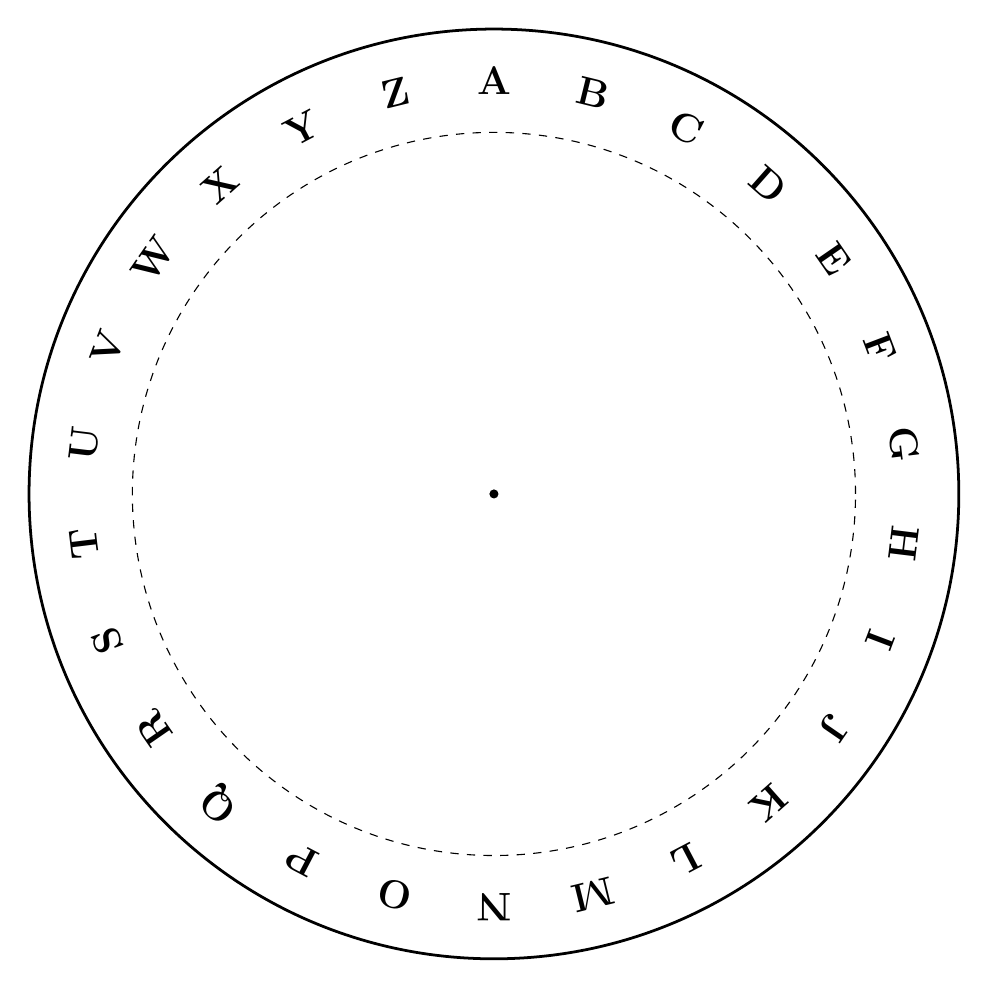
\begin{tikzpicture}[scale=0.82]
  \draw[line width=1pt] (0,0) circle (7.2);
  \draw[dashed] (0,0) circle (5.6);
  \foreach \l [count=\i from 0] in {A,B,C,D,E,F,G,H,I,J,K,L,M,N,O,P,Q,R,S,T,U,V,W,X,Y,Z}
    \node[font=\Large\bfseries,rotate={-\i*13.846}] at ({90-\i*13.846}:6.4) {\l};
  \fill (0,0) circle (2pt);
\end{tikzpicture}
\end{center}

\clearpage
\begin{center}
%% alt: The small inner circle of the letter-shift wheel, with the letters A to Z around its edge and a cutting line around it.
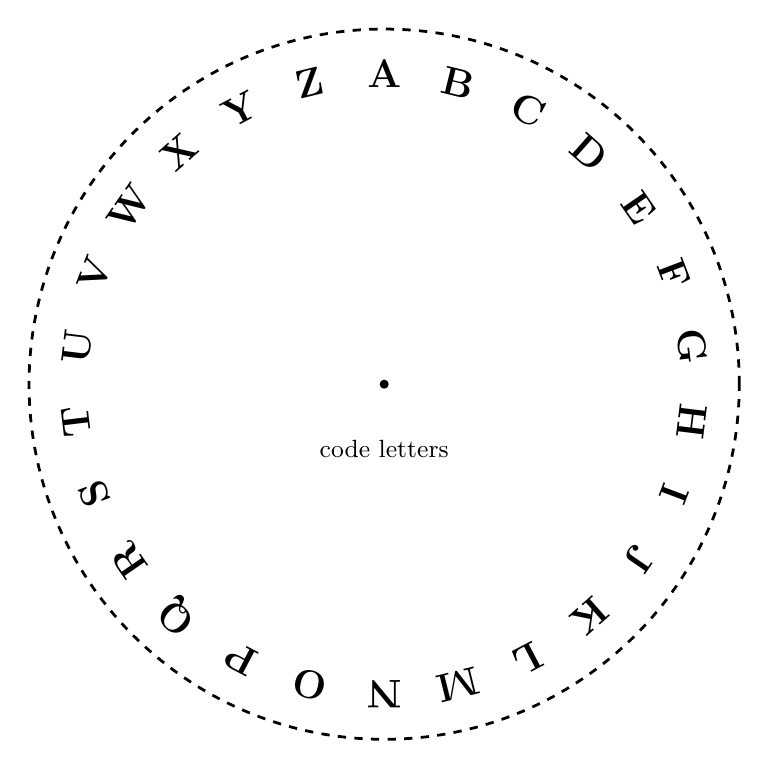
\begin{tikzpicture}[scale=0.82]
  \draw[line width=1pt,dashed] (0,0) circle (5.5);
  \foreach \l [count=\i from 0] in {A,B,C,D,E,F,G,H,I,J,K,L,M,N,O,P,Q,R,S,T,U,V,W,X,Y,Z}
    \node[font=\Large\bfseries,rotate={-\i*13.846}] at ({90-\i*13.846}:4.8) {\l};
  \fill (0,0) circle (2pt);
  \node[font=\small] at (0,-1) {code letters};
\end{tikzpicture}
\end{center}

\subsection*{Printable 3: the shift-3 strip (support path)}
Find your letter on the top row. Its code letter is underneath.
\begin{center}
\small\renewcommand{\arraystretch}{1.5}\setlength{\tabcolsep}{2.5pt}
\begin{tabular}{|*{13}{c|}}
\hline
A&B&C&D&E&F&G&H&I&J&K&L&M\\ \hline
\textbf{D}&\textbf{E}&\textbf{F}&\textbf{G}&\textbf{H}&\textbf{I}&\textbf{J}&\textbf{K}&\textbf{L}&\textbf{M}&\textbf{N}&\textbf{O}&\textbf{P}\\ \hline
\end{tabular}

\medskip
\begin{tabular}{|*{13}{c|}}
\hline
N&O&P&Q&R&S&T&U&V&W&X&Y&Z\\ \hline
\textbf{Q}&\textbf{R}&\textbf{S}&\textbf{T}&\textbf{U}&\textbf{V}&\textbf{W}&\textbf{X}&\textbf{Y}&\textbf{Z}&\textbf{A}&\textbf{B}&\textbf{C}\\ \hline
\end{tabular}
\end{center}

\subsection*{Printable 4: wheel messages and Zoe's card (shift 3)}
\begin{enumerate}[leftmargin=1.6em,itemsep=6pt]
  \item \textbf{SODB} \hfill \rule{5cm}{0.4pt}
  \item \textbf{BRX ZLQ} \hfill \rule{5cm}{0.4pt}
  \item \textbf{JRRG MRE} \hfill \rule{5cm}{0.4pt}
  \item \textbf{Zoe's card:} \enquote{I coded PLAY with shift 3. My code says SODC.} Which letter is wrong?
\end{enumerate}

\needspace{14\baselineskip}
\subsection*{Printable 5: logic puzzle cards (cut apart)}
\begin{enumerate}[leftmargin=1.6em,itemsep=6pt]
  \item \textbf{Pets.} Ada, Leo and Mei each have one pet: a cat, a dog or a fish. Clue 1: Ada's pet lives in water. Clue 2: Leo's pet does not say meow. Who has which pet?
  \item \textbf{Robot lights.} Rule: if the light is green, the robot moves 2 squares. If the light is red, the robot waits. The lights go: green, red, green, green. How many squares does the robot move?
  \item \textbf{Three chairs.} Kai, Zoe and Omar sit on three chairs: left, middle and right. Clue 1: Zoe sits in the middle. Clue 2: if Kai sits on the left, then Omar sits on the right. Clue 3: Kai does not sit on the right. Who sits where?
\end{enumerate}

\subsection*{Printable 6: treasure-hunt clue cards (four per pair)}
\begin{center}
\renewcommand{\arraystretch}{2.4}
\begin{tabular}{|p{6.5cm}|p{6.5cm}|}
\hline
Clue 1 (code: shift 3): & Clue 2 (code: shift 3): \\ \hline
Clue 3 (code: shift 3): & The treasure is here! \\ \hline
\end{tabular}
\end{center}
